\documentclass[12pt,a4paper,notitlepage,english]{article}
\usepackage[utf8]{inputenc}
\usepackage[title,titletoc,toc]{appendix}
\usepackage{amsmath}
\usepackage{amsfonts}
\usepackage{longtable}
\usepackage{wrapfig}
\usepackage{amssymb}
\usepackage{pdflscape}
\usepackage{hyperref}
\usepackage{graphicx}
\usepackage[a4paper, left=.5in,right=.5in,top=.5in,bottom=.5in,footskip=0.1in]{geometry}
\usepackage{tabularx,ragged2e,booktabs,caption}
\usepackage{setspace}
\usepackage[dvipsnames]{xcolor}
\usepackage[colorinlistoftodos,textsize=tiny]{todonotes}
\setstretch{1.5}
\usepackage{tabularx, booktabs}
\usepackage{dcolumn} 
  \newcolumntype{d}[1]{D{.}{.}{#1}}    
\newcolumntype{Y}{>{\centering\arraybackslash}X}
\usepackage[T1]{fontenc}
\usepackage{babel}
\usepackage{epigraph}
\usepackage{url}
\usepackage[citestyle=authoryear, style=apa, backend=biber, natbib]{biblatex}
\addbibresource{How_to_wage_a_trade_war.bib}
\newcommand{\source}[1]{\caption*{\footnotesize Source: {#1}} }
\usepackage{float}
\usepackage[section]{placeins}
\usepackage{ctable}
\newcolumntype{?}{!{\vrule width 2pt}}
 \newcolumntype{d}[1]{D{.}{.}{#1}} 
\DeclareUnicodeCharacter{202F}{ }
\usepackage{comment}
\begin{document}
\title{Not ``easy to win'':
The British war on French trade, 1716-1822}
\author{
  Guillaume Daudin \\ Université Paris-Dauphine \\guillaume.daudin@dauphine.psl.eu		
  \and
  Elisa Maria Tirindelli\footnote{This paper is not part of my PhD dissertation.} \\ Trinity College Dublin  \\ tirindee@tcd.ie
}
\date{}
\maketitle

%\section*{Abstract}

\epigraph{Savez-vous Messieurs ce qu’est une bataille navale ? On se rencontre, on se salue, on se canonne et la mer n’en reste pas moins salée.}{Maurepas, Navy Minister of Louis  \textsc{xv}, 1718-1748}

International trade is one of the main issues at stake in the rivalry between powers, to the extent that eighteenth-century Britons were much more preoccupied with war with France than with the Industrial Revolution.\footnote{Source: \href{https://books.google.com/ngrams}{Google NGrams}}
We know that in most situations war had a debilitating effect on trade \citep{karlsson2021war}. The mechanisms however are not clear.
World War I and World War II have shown that major powers can take quite a huge amount of punishment in terms of sunk tonnage before blockades endanger their economy. When it comes to eighteenth century wars however, the ratio between the value of the sailing ships and that of its cargo is several order of magnitude smaller. It follows that one had to destroy a larger number of them before the capital loss was noticeable from a macro perspective.  
And before the widespread use of submarines, the actual capacity of destruction of belligerents’ navy was not that big.
So what were the mechanisms that allowed Britain to achieve its mercantilist war goals in this settings?
Mercantile rivalry was an important motivation of war all throughout the eighteenth and nineteenth century (\citet{wallerstein_modern_1980, crouzet_guerre_2008}). In fact, both the British and the French believed it was a good way to curtail enemy's trade, albeit the French were more wary of wars because they did not have much naval success.\\
\begin{figure}
\caption{French, British trade and Anglo-French wars}
\centering
\label{FrBritTrade}
%\begin{minipage}[t]{0.9\textwidth}
%\raggedright
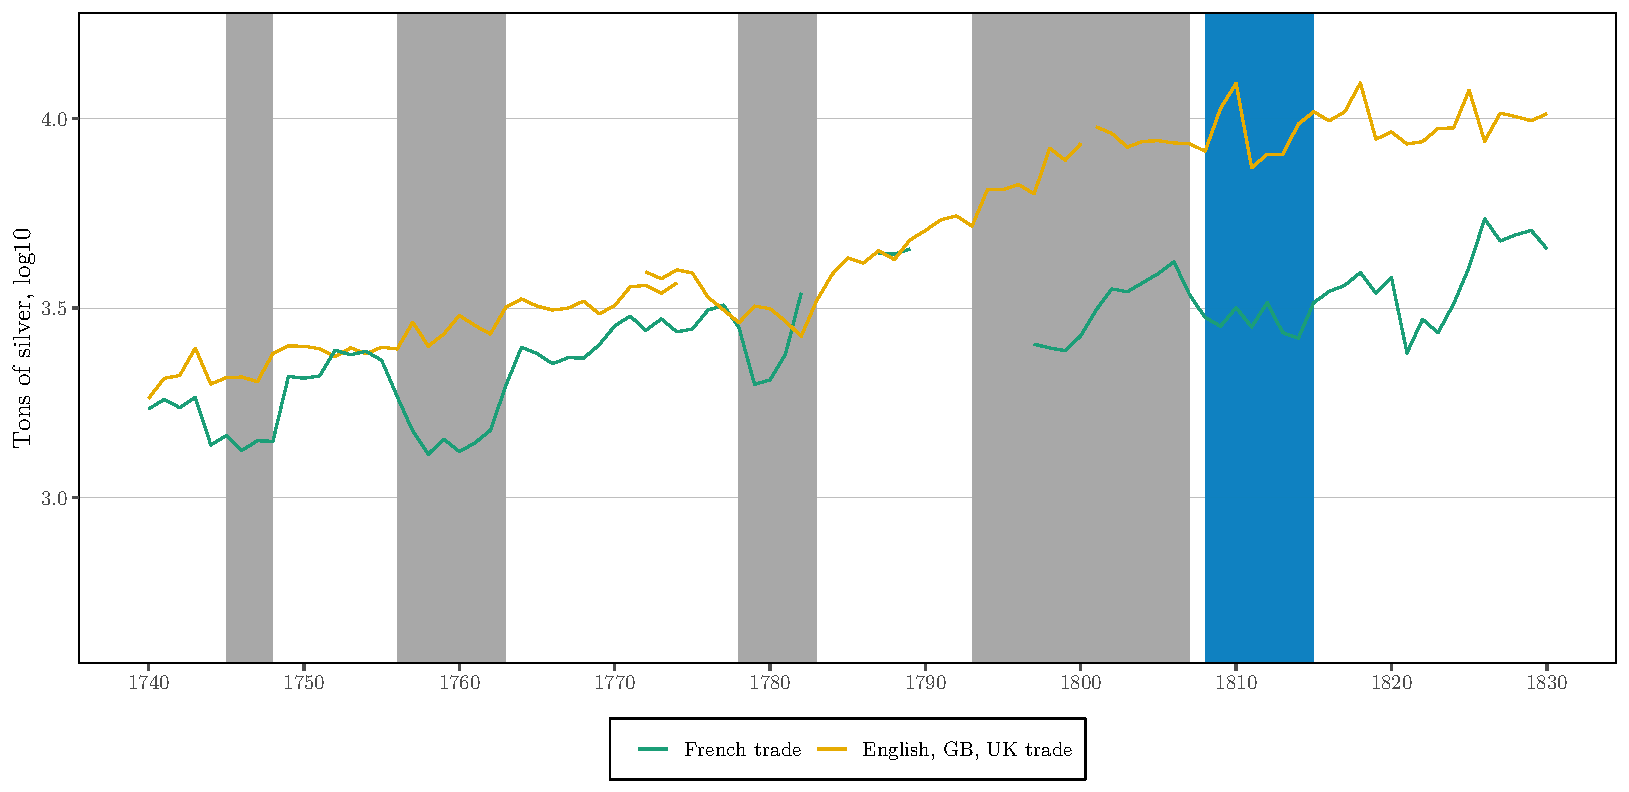
\includegraphics[scale = .6]{Total_silver_trade_FR_GB.pdf}
%{\scriptsize \source{French trade up to 1821: \citet{daudin_toflit18_????}. French trade 1822-1840: \cite{federico_world_2016}  \citet{dedinger_exploring_2017},
%England/British trade up to 1800: \citet{deane_british_1969}. UK trade from 1801 to 1840: \cite{federico_world_2016} / \citet{dedinger_exploring_2017},
%Livre tournois silver value: \citet{de_wailly_memoire_1857} and \citet{hoffman_priceless_2000}; Pound sterling silver value: \citet{clark_england_1209-1914_2006} and \citet{jastram_silver_1981}}\par}
%\end{minipage}
\end{figure}
It is not obvious whether and how any of the long list of wars between France and Britain after the death of Louis XIV achieved their mercantile goal effectively.
Figure \ref{FrBritTrade} shows that French trade, despite a decrease in wartime, was recovering quite fast after many wars.
Computing a loss function for French trade reveals a more detailed picture.
Loss is defined as the percentage loss of trade compared to past peace time trend:
\begin{equation*}
Loss = \frac{\text{Expected value based on past peace trend - Observed value}}{\text{Expected value based on past peace trend}}
\end{equation*}
Figure \ref{fig:mean_annual_loss} shows the annual and mean loss function.
It is evident that the peace percentage loss of the Seven Years Wars and that of the Napoleonic Wars were comparable to wartime loss, as opposed to faster recoveries in other post-war periods.
What made these wars so effective in terms of trade disruption?
To answer this question we first distinguish between ``wartime strategies'' (ship building and alliance making, capture of colonies, predation on enemy's shipping, predation on neutral shipping ) and ``peace-time strategies'' (log-term trade restructuring), we then provide a measure to quantify their success and finally we establish a link with the loss function to draw conclusions. 

We start by analysing the ``wartime strategies''. 
To have a sense of the superiority of the British navy over its enemies, we compare the number of warships available to Great Britain and its allies with that available to France and its allies, as provided in \citet{modelski1988seapower}.
From this comparison we learn that the most favourable war for France, its allies and neutral countries was the Seven Years War, when the number of neutral warships or ships on the French side was more than twice as much that of Britain and its allies.
This suggests no clear relationship with the loss function and the supremacy of the British navy. \\
\begin{figure}
    \centering
    \caption{Loss Function}
    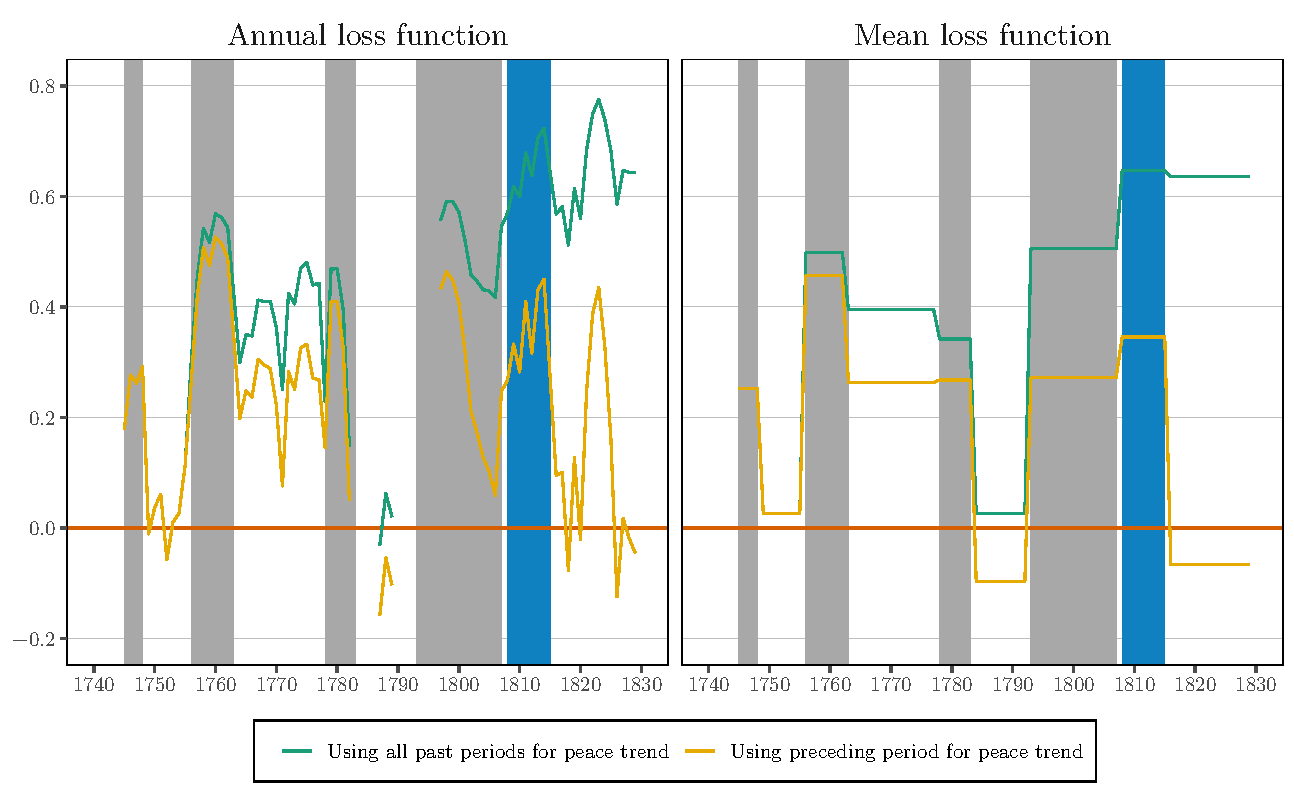
\includegraphics[scale = .7]{mean_annual_loss.pdf}
    \label{fig:mean_annual_loss}
\end{figure}
Capture of colonies was strategic as West Indian French colonies were a major source of production of colonial goods to be imported and then re-exported by France to other European countries. Their loss was bound to be disruptive for French trade, as it reduced both imports and re-exports.
We provide a measure to quantify the importance of this source of trade, by observing the evolution of the extension of the colonial empire, weighted by share of total trade. We find that, even if the loss of colonies had a large effect on French trade, this was not enough to make a successful trade war. For example, it does not explain why trade losses were so large after the Seven Years War, even though the West Indian French colonies were not lost. \\
Predation on shipping was a substantial threat to trade during trade wars. Great Britain had three ways of affecting sea trade: outright destruction of merchant vessels, ransoming, and prize taking. Because direct destruction was rare and ransoming was limited, the overall value of prizes captured by the British navy and privateers provides a good measure of the the pressure war-time predation exerted on trade. Data from \citet{Benjamin2009} and \citet{Hillmann2011} on prizes captured by the English navy show that lost French shipping was much higher during the War of American independence than during the Seven Years War, even though the latter had more severe effects on French trade.\\
Finally, the role of neutrals during wars, and especially during trade wars, was very important. On the one hand they were the only ones who could provide goods that were not otherwise available due to the war \citep{Hedberg2015}. On the other hand, they were an expedient for merchants who hid their cargoes as neutral cargo and could continue to trade. (see \citep{carriere1973negociants}, \cite{schnakenbourg2013guerre}). A tentative quantification of the variation in policy towards neutral trade shows that French trade losses are well correlated with the degree of hostility shown by both France and Britain toward neutral trade.
In fact, during the Seven Years War, the British introduced the \textit{Doctrine of Continuous Voyage} along with the \textit{Rule of War of 1756}, that was an important step against neutral trade in wartime. 
Also, in the Revolutionary \& Napoleonic wars, France itself became more and more hostile to neutral shipping as a way to try and isolate Great Britain, therefore, at that time, neutral trade was opposed by the two major European powers.  \\
Of the four ``wartime strategies'' analysed, the latter is the one that best explains the loss function, therefore we argue that for a trade war to be successful it was necessary to disrupt neutral trade. \\
\begin{figure}
    \centering
    \caption{Ratio between French trade losses and the British Navy budget, high and low hypothesis}
    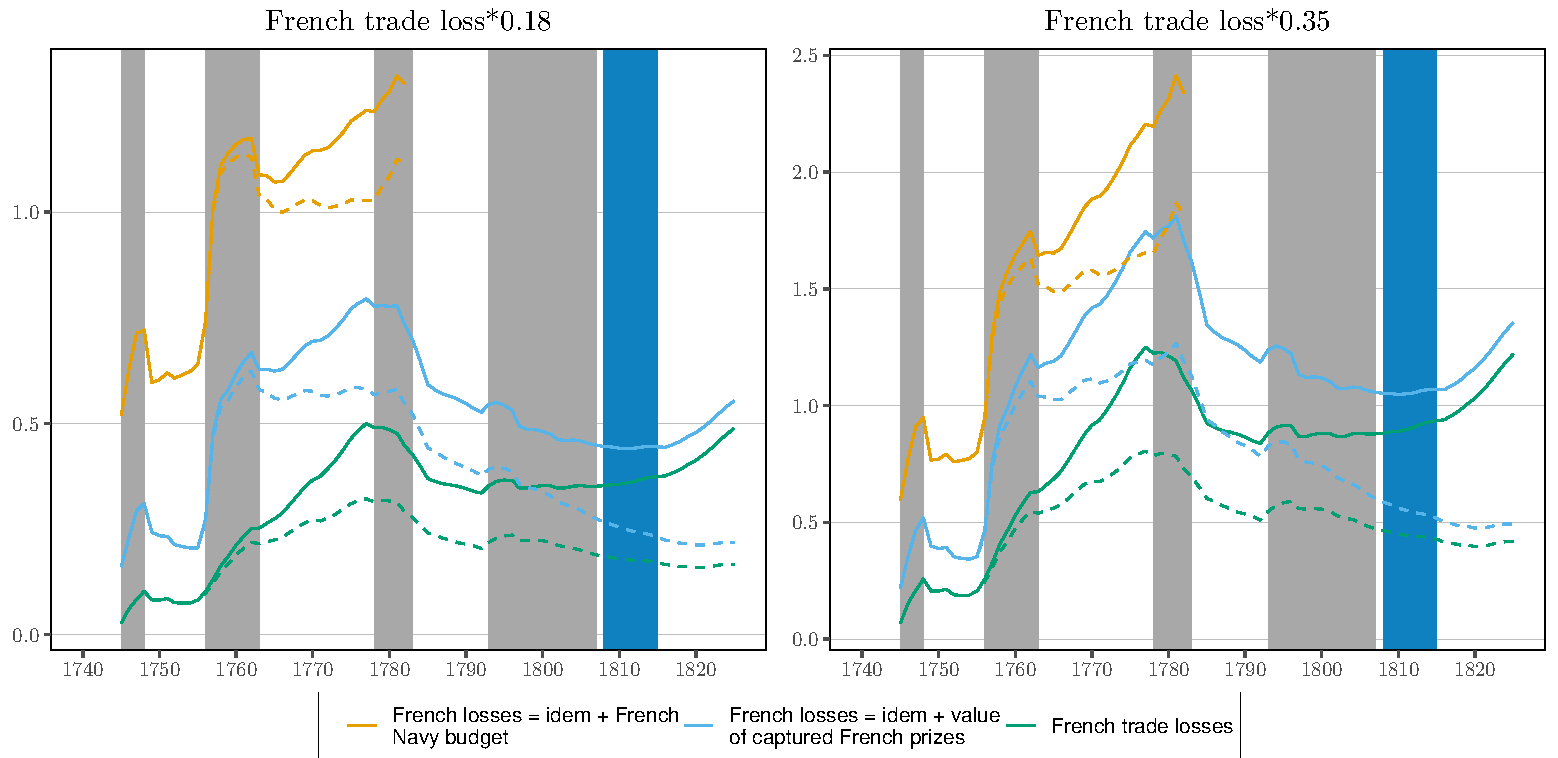
\includegraphics[scale = .6]{ratio_BR_expenditures_ennual_loss.pdf}
    \label{fig:ratio_BR_expenditures_annual_loss}
\end{figure}
We now want to disentangle the underlying mechanisms.
Our hypothesis is that trade wars were successful when they imposed lasting changes in trade structure.
We run different linear regressions of the loss function on the share of each product and of trade to each country, exploiting new data from the \href{https://toflit18.hypotheses.org}{TOFLI18} database.
We show that, even when controlling for a time trend and the contemporaneous effect of war, the changing level of total French trade losses is associated with changes in the industrial structure of trade. We find similar changes in the partner share of French trade in the regional share of French trade up to 1789. 
This does not statistically establish causality.
Yet, the most plausible channel explaining these findings is that ``successful'' wars (from the British point of view) transformed the structure of French trade.
These transformations were difficult to reverse after the wars and French trade was durably locked into a less dynamic structure. \\
This transformation of the French economy took a long time to achieve for Britain and obviously came at a cost. Albeit complex, we try to quantify the cost of the trade war for Britain compared to the losses for France.
%To some extent, it was only possible because Napoleon cooperated with Britain in transforming the French economy by using external trade as a tool to exploit Europe for the French advantage through the continental system.
We are careful to recognize that reduced trade cannot be compared directly with the British cost of waging war on French trade.
Using \citet{Daudin2005}, we evaluate the income lost to France as a share of lost trade.
On the balance sheet, we put the French and British naval budget, the value of British and French prizes and outfitting cost by privateers in both countries.
If one assumes that France was able to re-integrate in the French economy the production factors made idle by the trade loss, albeit at a lower productivity, it is not clear that French losses were much higher than the cost incurred by Britain to wage war.
Even being more optimistic, the cost of naval war as a share of British GDP was certainly smaller than French losses as a share of French GDP (see figure \ref{fig:ratio_BR_expenditures_annual_loss}). 

We can conclude that waging war on France did allow Britain to reduce the long-term openness of France and contributed to transforming France into a relatively inward-looking economy in the nineteenth century.
That effort required steady and costly effort by Britain to permanently change French trade industrial and geographical structure.
The harsh treatment of neutral trade (which, when possible, allowed French trade to adapt nimbly to war) made an important contribution to British achievements.
This had an important geopolitical cost, leading for example to to war with Spain in 1762 and with the USA in 1812, which is not factored in our cost-benefit analysis.
French cooperation were paradoxically also central in achieving British mercantile war aims.



\textbf{Keywords}: international trade, 18th century, France, neutral trade, trade war

%\pagebreak

\renewcommand{\baselinestretch}{1.0}\normalsize
\printbibliography

%\bibliographystyle{apalike}
%\bibliography{How_to_wage_a_trade_war}

\end{document}